\chapter{Methodology}
\label{chapter:chapter03}

In the following chapter is explained the different parts of the problem to solve and...

\section{Problem Design}

The problem established is described as given a data set $D$ of $n$ students $D = (s_1,...,s_n)$, A solution $A$ consists of an optimal arrangement of groups $G$, this arrangements assigns each student to a group $A = \langle s_i \leftarrow G_j, s_n \leftarrow G_m...  \rangle$, with the students being in the same group optimising their preference criteria as described in \ref{chapter:chapter02}, this optimisation is described as finding the less distance between the level of experience of the students inside the same group , finding the less distance among an ontology of interests, where similar interests related interests are in the same branch, as well as the having a group size near the optimal group size which is defined as between 4 and 5, and the percentage of participation which is how much the students participate in the conversation of the group, maximising for the most participation.\\

The solution is then the number of the group for each user, serving it as an id only, without any relevance in the order the groups are presented, only that the preference of the users is maintained within the group, this can more clearly be seen in figure \ref{dataset_eg} and equation \ref{eq:students_groups}.\\

The problem was approached in two different ways, considering the groups as the variables and the students as the values, and the other way around, considering the students as the variables and the groups as the values. The former approach had the disadvantage that the number of variables was inconsistent depending on the size of the groups, and that reflected at the moment of testing the algorithms, because most of have a crossover and mutation rate related to the size of the variables, another disadvantage was that some groups could remain empty and the crossover and mutation added unnecessary complexity to the task.\\

In addition a linked list is kept in order to keep track of the groups internally and make the evaluation of objective functions easier, which means if $s_i \leftarrow G_j$ then $G_j = (...,s_i,...)$

The search space comprehends all the possible assignments of groups to the students, which means that is roughly $(n/n!)$, for a solution $S$, the neighbourhood is composed by every solution that has a single student in a different group, among the feasible solutions.

\begin{figure*}
    \caption{This is an example of a data set of 9 users, each with their experience, 3 different interests and a participation percentage, as it can be seen the Group $G_3$ is assigned to students according to the preference criteria.}
    \label{dataset_eg}
    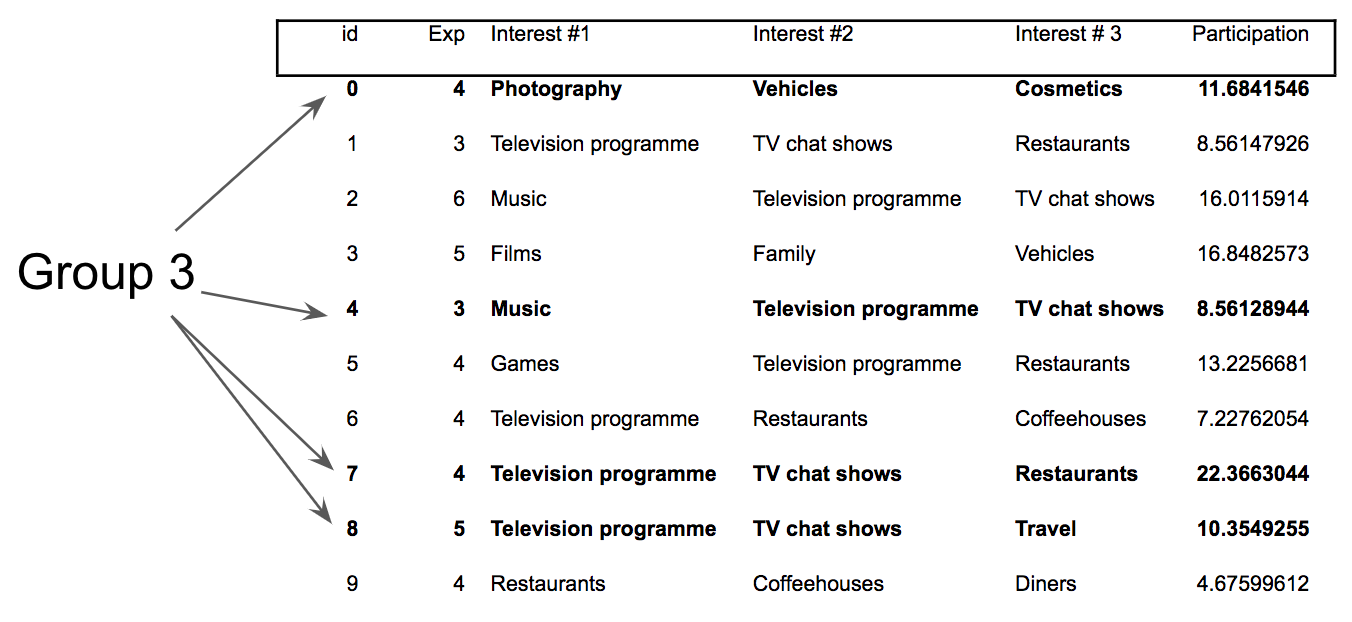
\includegraphics[width=0.85\textwidth]{images/dataset_eg.png}
\end{figure*}

\begin{equation*}
  \label{eq:students_groups}
  \begin{gathered}
        D = (s_0,s_1,s_2,s_3,s_4,s_5,s_6,s_7,s_9,...,s_n),\\
        A = \langle s_0 \leftarrow G_3, s_1 \leftarrow G_0, s_2 \leftarrow G_2,     s_3 \leftarrow G_1, s_4 \leftarrow G_3, s_5 \leftarrow G_1,...  \rangle
  \end{gathered}
\end{equation*}

\section{Objective Functions}

In the following section, the different objective functions are described, this are proposed according to the preference criteria defined in \ref{chapter:chapter02}.


\subsection{Tamaño del Grupo}

Para propósitos de la investigación el tamaño ideal del grupo se considera como de \textbf{4 a 5} personas, ya que este tamaño usualmente permite una participación de todos los usuarios que pertenezcan al grupo. Es posible que puedan existir grupos de \textbf{3 o 6} personas, pero esto no es lo ideal, sin embargo se deja abierta la posibilidad en caso de que alguna otra característica como los intereses en común o el estilo de participación resulten más relevantes para el grupo que su tamaño.

La función para calcular este objetivo mide la cercanía al valor \textbf{4.5}, ya que 4 y 5 se consideran igual de ideales y 4.5 es simplemente el promedio entre ambos valores. Esta función esta definida a continuación:\ref{eq_group_size}

\begin{equation} \label{eq_group_size}
    f = | groupSize - 4.5|
\end{equation}

\subsection{Nivel de experiencia}

El nivel de experiencia en el lenguaje hace referencia al estándar CEFR\cite{}. Los valores que se consideran para ello son A1, A2, B1, B2, C1 y C2, por lo que se les asigna un valor numérico a cada uno siendo A1 0 y C2 5. Lo que se busca principalmente es que los usuarios dentro del grupo no tengan mucha variación en cuanto a su nivel de experiencia. De esta forma el vocabulario usado no se considera tan avanzado para integrantes con un nivel bajo ni tan sencillo para integrantes más avanzados. La fórmula\ref{eq_nivel} consiste en una desviación estándar del valor del nivel de cada uno de los integrantes, de forma ideal que sea alcanzado el 0 indicando que todos los usuarios del grupo forman parte del mismo.

\begin{equation} \label{eq_nivel}
    \sigma = \sqrt{\frac{1}{n-1} \sum_{i=1}^n (x_i - \overline{x})^2}
\end{equation}

\subsection{Intereses}

Para calcular la similitud entre intereses se usa una estrategia similar a Madylova y Gunduz \cite{taxonomy_semantic_similarity} donde los intereses son considerados como un vector valores en los que se señala una cantidad que indica el orden jerárquico de acuerdo a la ontología definida por la red social de Facebook, por ejemplo si un usuario tiene como intereses: Los perros, Correr y las Citas, su vector de intereses se estaría dado por los valores en la Figura \ref{fig:interests_table}. En la parte de arriba se indica el valor de la jerarquía, en la parte de abajo se normaliza usando $1/(1+v)$, después se eligen los valores mayores de cada una de las columnas de esta forma da el vector resultante como se muestra en la Figura \ref{fig:interests_vector} \\

\begin{table}[]
\caption{Interests mapping of a $s_1$ example user}
\label{tab:interests_s_1}
\centering
\begin{tabular}{|c|c|c|c|c|c|c|}
\hline
                & Interests & Business & Design   & Graphic Design & Interior Design & Banking  \\ \hline
Graphic Design  & 3         & 2                     & 1        & 0              & $\infty$        & $\infty$ \\ \hline
Interior Design & 3         & 2                     & 1        & $\infty$       & 0               & $\infty$ \\ \hline
Banking         & 2         & 1                     & $\infty$ & $\infty$       & $\infty$        & 0        \\ \hline
                &           &                       &          &                &                 &          \\ \hline 
Graphic Design  & 0.25      & 0.333...              & 0.5      & 1              & 0               & 0        \\ \hline
Interior Design & 0.25      & 0.333...              & 0.5      & 0              & 1               & 0        \\ \hline
Banking         & 0.333...  & 0.5                   & 0        & 0              & 0               & 1        \\ \hline
\end{tabular}
\end{table}


\begin{table}[]
\caption{Interests mapping of a $s_2$ example user}
\label{tab:interests_s_1}
\centering
    \resizebox{\textwidth}{!}{
        \begin{tabular}{|c|c|c|c|c|c|c|c|}
        \hline
                        & Interests & Business & Advertising & Banking  & Retail Banking & Hobbies  & Running  \\ \hline
        Graphic Design  & 3         & 2        & $\infty$    & 1        & 0              & $\infty$ & $\infty$ \\ \hline
        Interior Design & 2         & 1        & 1           & $\infty$ & $\infty$       & $\infty$ & $\infty$ \\ \hline
        Banking         & 3         & $\infty$ & $\infty$    & $\infty$ & $\infty$       & 1        & 0        \\ \hline
                        &           &          &             &          &                &          &          \\ \hline
        Graphic Design  & 0.25      & 0.333... & 0           & 0.5      & 1              & 0        & 0        \\ \hline
        Interior Design & 0.333...  & 0.5      & 0.5         & 0        & 0              & 0        & 0        \\ \hline
        Banking         & 0.25      & 0        & 0           & 0        & 0              & 0.5      & 1        \\ \hline
        \end{tabular}
    }
\end{table}

\begin{table}[]
\caption{Interests mapping of a $s_2$ example user}
\label{tab:interests_s_1}
\centering
\resizebox{\textwidth}{!}{
    \begin{tabular}{|c|c|c|c|c|c|c|c|c|c|}
    \hline
          & Interests & Business & Design & Graphic Design & Interior Design & Banking & Retail Banking & Hobbies & Running \\ \hline
    $s_1$ & 0.75      & 0.5      & 0.5    & 1              & 1               & 1       & 0              & 0       & 0       \\ \hline
    $s_2$ & 0.33      & 0.5      & 0      & 0              & 0               & 0.5     & 1              & 0.5     & 1       \\ \hline
    \end{tabular}
}
\end{table}

Para calcular que tan similar es un usuario con respecto a otro se usa la formula de distancia cosenoidal, que se muestra en la ecuación \ref{eq_cos_sym} donde \(A\) es el vector de intereses del primer usuario y \(B\) es el vector de intereses del segundo. Cabe destacar que es muy frecuente que los vectores de intereses de los usuarios contengan ceros al momento de compararlos, de tal manera que si el resultado de la función da como resultado exactamente 0, significa que ambos usuarios no tienen nada en común. 

\begin{equation} \label{eq_cos_sym}
    \cos(\theta) = \frac{ \sum\limits_{i=1}^{n}{A_i  B_i} }{ \sqrt{\sum\limits_{i=1}^{n}{A_i^2}}  \sqrt{\sum\limits_{i=1}^{n}{B_i^2}} }   
\end{equation}
\begin{equation}\label{eq_interests}
	f = 1 - \cos(\theta) 
\end{equation}

\subsection{Estilo de Participación}

Para esta función trato de buscarse en la literatura algún tipo de función matemática ya definida para evaluar que tipo de roles son los que provocan que haya una participación más homogénea dentro del grupo dependiendo del rol funcional de cada uno de los participantes y su compatibilidad entre si. Sin embargo no se encontró ninguna, por lo que fue necesario definirla por medios propios. Afortunadamente se cuenta con una definición concreta de como debe ser la función, tomar en cuenta como parámetro los roles funcionales de cada usuario y dando como resultado de su evaluación el nivel de participación del grupo de forma numérica con la idea de optimizar dicho resultado.

Es por esto que al hacer el análisis de los datos como se describe en la sección de Experimentación [ref], se toman en cuenta 

%Ya que no hay ningún paper que diga que función usar para esto se le hizo un análisis de datos al AMI meeting corpus para ver que relación había entre el número de silencios y la homogeneidad de las participaciones de acuerdo con los funcional roles de Benne & Sheats, y pues resulta que si hay una correlación con respecto al porcentaje de participaciones por lo que se uso esta medida para tratar de predecir la interacción del grupo, considerando que esta participación debe ser homogénea entre ellos por lo que es el inverso a la suma de las participaciones y así...

% - Esta función está pensada para que pueda haber fluidez para hablar dentro del grupo; minimizando los silencios y aumentando volviendo el número de participaciones uniforme con respecto a los usuarios.
% - Hay mucha literatura mencionando porque esto funciona, pero nadie dice una medida matemática que se pueda usar para esto...
% - Se hizo un análisis de los datos a la base de datos de AMI, y se descubrió que los silencios y las participaciones están directamente relacionados con respecto a una medida de participación dentro del grupo, en efecto, se necesita.
% - TODOS los usuarios se comportan como protagonistas en algún punto, ya que este es el estilo que nos interesa optimizar es en el que nos basamos.
% - Más adelante al momento de generar la base de datos esto también hace sentido y así... 

\section{Operators}

This next section describes the different operators applied by the algorithms to the solutions, in the case of meta-heuristics like LC or PT, where in each iteration a step in the search space is perform, the operator of mutation is used, and for the case of RD which requires all a defined neighbourhood all the possible mutations are used. For the genetic algorithms and other evolutionary strategies a crossover operator is also used. The same mutation and crossover operators are used for all the algorithms that allow them.

\section{Initialisation}

All the algorithms start with a random initial population, first, the groups are generated according to the maximum possible groups which is $(\lfloor\frac{n}{gs_{min}}\rfloor)$, this groups are stored in a vector $AG$ which comprehend the available groups, when a group is filled, that means has reached the $gs_{max}$ number of students leaves the vector $AG$, if a move is performed by the operators and the group misses a student, then this group returns to the $AG$ vector.\\

Then each student is assigned to a random group from $AG$, to prevent the solutions becoming unfeasible, that is, for example if a single student is left alone in a group, a $Repair$ operator is applied after the initialisation, this is defined later in this section. This completed process is defined in algorithm \ref{alg:initialisation}.

\begin{algorithm}[H]
\caption{Initialisation}
\label{alg:initialisation}
\SetAlgoLined 
$AG \leftarrow$ Create $(\lfloor\frac{n}{gs_{min}}\rfloor)$ groups;\\
\For{$s_i \in D$}{
    $s_i \gets G \in AG$ \Comment Assign a random group to $s_i$\;\\ 
    $A \gets s_i$
}
Perform $Repair$ in $A$
\end{algorithm}

\subsection{Mutation}

Una mutación de acuerdo a los algoritmos genéticos debe de introducir al sistema una solución que no se exista aún. Sin embargo no es suficiente con cambiar un usuario por otro en un grupo para la mutación ya que este usuario probablemente se encuentre en otro grupo diferente y el sistema prohíbe que un usuario este en 2 grupos distintos a la vez. Por ello el algoritmo para la mutación toma un grupo de origen al azar, quita un usuario de un grupo y lo pone en otro, tomando en cuenta las restricciones del tamaño del grupo, es decir, si es un grupo que quitándole un usuario resultaría menor a 3 entonces se debe seleccionar otro grupo. De forma similar para el grupo destino se verifica que no sobrepase el tamaño máximo de 6 una vez que el nuevo usuario sea agregado, y si es el caso se selecciona otro grupo. El algoritmo completo se presenta como pseudocódigo a continuación:

jMetal cuenta con distintos algoritmos para realizar la mutación, sin embargo estos comprenden únicamente problemas binarios o de permutación, y ya que es necesario un algoritmo para obtener una solución combinatoria, fue necesaria la creación de un nuevo algoritmo que a continuación se propone.

For the mutation task, a individual value of the solution set is changed to another group

\begin{algorithm}[H]
    \caption{Group Swap mutation}
    \label{alg:mutation}
    \SetAlgoLined 
    Get a random student $s_i \in A$\;\\
    Get a random group $G_j \in AG$\;\\
    $s_i$ \gets $G_j$ \Comment{Assign $G_j$ to $s_i$}
\end{algorithm}

\begin{figure}
    \centering
    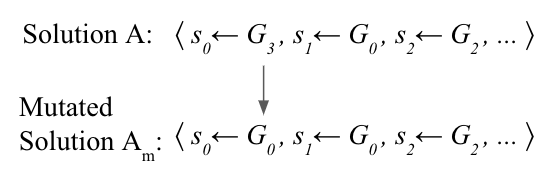
\includegraphics[width=0.8\textwidth]{images/mutation_g.png}
    \caption{Caption}
    \label{fig:my_label}
\end{figure}

% ASK: 

\subsection{Crossover}

La herramienta de jMetal cuenta con distintos algoritmos de crossover, y ya que estos únicamente se basan en los cromosomas que corresponden a los grupos creados, es posible usar cualquier algoritmo de esta herramienta para generar soluciones nuevas en la población. El algoritmo que se usó en cuestión recibe el nombre de N-Point Crossover, donde la N corresponde al número de cromosomas que se cruzaran, es decir suponiendo que n = 10 entonces 10 grupos se tomarán de una solución y se pasarán a otra que a su vez también intercambiará 10 grupos y el resto... ya que se busca que el crossover se realice justo a la mitad, esta N corresponde al número de cromosomas/variables o bien el número de grupos.

Para la primera fase los experimentos que se definieron consistieron en probar únicamente las funciones objetivo de forma individual y determinar su factibilidad con respecto a si son reproducibles y pueden ser útiles para cualquier tipo de solución generada.

\begin{algorithm}[H]
    \caption{K-point Crossover}
    \label{alg:crossover}
    \SetAlgoLined 
Select two parents $A$ and $B$ from a parent pool\;\\
Create two offspring $C$ and $D$ a follows:\;\\
Randomly choose $k$ crossover points $cp_1,...cp_k \in {1,...,n-1}$\;\\
\For{$i \gets 1$ to $cp_1$}{
    $c_i \gets a_i$\;\\
    $d_i \gets b_i$
}
$switch \gets 0$
\For{$j \gets 2 to k$}{
    \eIf{$switch = 0$}{
        \For{$i \gets cp_{j-1} + 1$ to $cp_j$}{
            $c_i \gets b_i$\;\\
            $d_i \gets a_i$
        }
        $switch \gets 1$        
    }{
        \For{$i \gets cp_{j-1} + 1$ to $cp_j$}{
            $c_i \gets a_i$\;\\
            $d_i \gets b_i$
        }
        $switch \gets 0$        
    }
}
\eIf{$switch = 0$}{
    \For{$i \gets cp_{j-1} + 1$ to $cp_j$}{
        $c_i \gets b_i$\;\\
        $d_i \gets a_i$
    }
}{
    \For{$i \gets cp_{j-1} + 1$ to $cp_j$}{
        $c_i \gets a_i$\;\\
        $d_i \gets b_i$
    }
}
Perform $Repair$ in $C$ and $D$
\end{algorithm}

\begin{figure*}
    \centering
    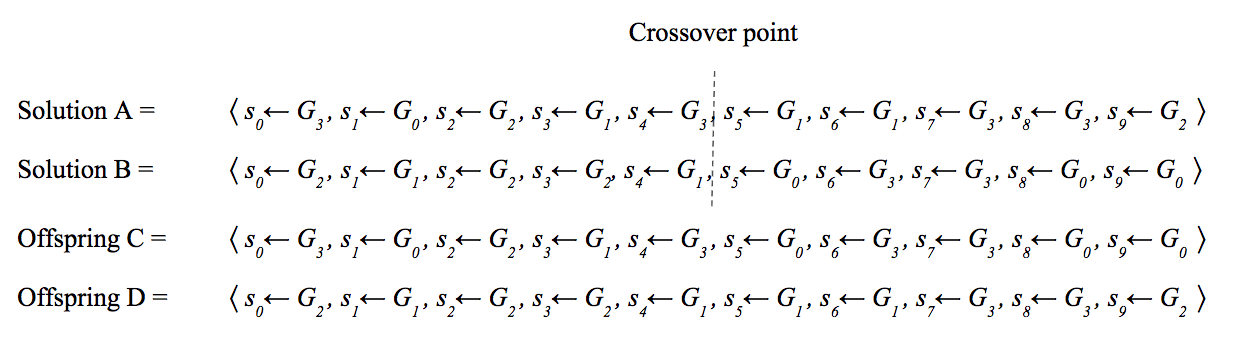
\includegraphics[width=1.1\textwidth]{images/cross_over_g.png}
    \caption{Caption}
    \label{fig:my_label}
\end{figure*}


\subsection{Repair}

Is possible that after performing the crossover operation, either a group ends up with a higher number of students than the allowed $gs_{max}$ or a smaller number $gs_{min}$, for this reason a repair procedure is performed after the initial population and after each crossover, to make sure the solutions produced remains within the problem constraints.\\

The algorithm consists of checking each group size, if the size is higher than $gs_{max}$, then its split in half, if the size is lower than $gs_{min}$ then it requires more members to be feasible and is marked as a pending group $P_g$, therefore after a group $G_i$ with $Size(G_i) > gs_{max}$ is found a user from $G_i$ is assigned to $P_g$, and the algorithm continues until all the groups become feasible.
The fill algorithm can be seen in \ref{alg:repair}

\begin{algorithm}[H]
    \caption{Group Repair}
    \label{alg:repair}
    \SetAlgoLined 
    $A_r = ()$\;\\
    $P_g \leftarrow NULL$\;\\
    \For{$ G_i \in A$}{
        \If{$Size(G_i) > 0$}{
            \If{$P_g$ is not $NULL$ $\textbf{AND}$ $Size(P_g) \leq gs_{max}$ $\textbf{AND}$ $Size(P_g) > gs_{min} $}{
                $A_r \gets MergeGroups(P_g,G_i)$\;\\
                $P_g \leftarrow NULL$
            }\;\\
            \If{$Size(G_i) < gs_{min}$}{
                $A_r \leftarrow SplitGroup(G_i)$ \Comment{Split $G_i$ the group in half}
            }\;\\
            \eIf{$Size(G_i) > gs_{max}$}{
                $P_g \leftarrow G_i$ 
            }{
                $A_r \leftarrow G_i$
            }
        }
    }
\end{algorithm}

% Synthetic Dataset?